\chapter{Diseño e implementación} % Main chapter title

\label{Chapter3} % Change X to a consecutive number; for referencing this chapter elsewhere, use \ref{ChapterX}

En este capítulo se describe el diseño y la implementación de la solución desarrollada para automatizar el pronóstico de la demanda eléctrica del SADI. En primer lugar, se presenta el pipeline implementado para obtener, validar, transformar y almacenar los datos de demanda y las variables meteorológicas utilizadas por los modelos. A continuación, se describen la arquitectura de los modelos, el procedimiento de entrenamiento y optimización, y los mecanismos empleados para generar y persistir las predicciones. Finalmente, se detalla la integración de estos componentes en el sistema implementado, junto con las decisiones adoptadas para garantizar la trazabilidad y la reproducibilidad de las ejecuciones.

%----------------------------------------------------------------------------------------
% CAPÍTULO 3.1: PIPELINE DE DATOS
%----------------------------------------------------------------------------------------
\section{Pipeline de datos}
\label{sec:pipeline_datos}
%----------------------------------------------------------------------------------------

El sistema de pronóstico requiere integrar series eléctricas, meteorológicas y calendarias con diferentes resoluciones temporales, coberturas geográficas y mecanismos de acceso. Por este motivo, antes de abordar la construcción y evaluación de los modelos se diseñó un pipeline de datos que automatiza la extracción, el procesamiento, la validación y la persistencia de la información. El objetivo de esta etapa fue disponer de conjuntos de datos consistentes y trazables, adecuados tanto para el entrenamiento como para la ejecución periódica de pronósticos.

La solución se implementó sobre la arquitectura híbrida presentada en el capítulo~\ref{Chapter2}. Los procesos que necesitan conectividad con sistemas internos de CAMMESA se ejecutan en un servidor local mediante Dagster. El almacenamiento y las transformaciones posteriores se concentran en Microsoft Fabric, donde se utilizan una base de datos KQL para la recepción inicial de determinados datos, un Data Warehouse para las capas estructuradas y Pipelines y notebooks para la orquestación y el procesamiento. Esta separación evita exponer directamente las fuentes internas y, al mismo tiempo, centraliza en Fabric la información utilizada por los modelos.

El pipeline se organizó en tres flujos principales, que obtienen y transforman los siguientes grupos de variables:

\begin{enumerate}
	\item Demanda eléctrica.
	\item Datos meteorológicos reales.
	\item Pronósticos meteorológicos. 
\end{enumerate}

La información calendaria se incorpora posteriormente mediante tablas de existentes en las bases de datos de CAMMESA, de modo que pueda combinarse con las series eléctricas y meteorológicas utilizando la fecha como clave temporal.

%----------------------------------------------------------------------------------------
\subsection{Criterios de diseño del pipeline}
\label{subsec:criterios_pipeline}
%----------------------------------------------------------------------------------------

El diseño se basó en cuatro criterios. En primer lugar, se buscó reducir la intervención manual en la obtención y actualización de datos. Las tareas repetitivas se encapsularon en activos de Dagster, notebooks y actividades de Pipeline, según el entorno desde el cual debía accederse a cada fuente. En segundo lugar, se preservó la granularidad original durante las primeras etapas. La demanda se almacena inicialmente con resolución de diez minutos y los datos meteorológicos conservan las resoluciones horaria o diaria provistas por cada fuente. Las agregaciones necesarias para el modelado se realizan en capas posteriores.

En tercer lugar, se incorporaron controles de calidad antes de generar las variables de entrenamiento. Estos controles abarcan la completitud temporal, la coherencia entre la demanda nacional y la suma regional, la consistencia de la partición de la provincia de Buenos Aires y la identificación de valores anómalos en las series horarias. Finalmente, se separaron los datos originales de los valores corregidos. Esta decisión permite conservar trazabilidad sobre las transformaciones y distinguir los registros que requirieron tratamiento.

La persistencia se estructuró mediante capas. La capa~1 recibe datos con un grado mínimo de elaboración y conserva una representación cercana a la fuente. La capa~2 contiene información validada, tipificada e integrada. Sobre estas tablas se construyen vistas y conjuntos derivados orientados al consumo analítico y al modelado. Esta organización evita aplicar transformaciones irreversibles durante la ingesta y facilita repetir los procesos cuando se modifican las reglas de limpieza.

%----------------------------------------------------------------------------------------
\subsection{Ingesta de demanda desde el SOTR}
\label{subsec:ingesta_demanda_sotr}
%----------------------------------------------------------------------------------------

La demanda eléctrica se obtiene desde PI System mediante PIconnect. Debido a que esta fuente solo es accesible desde la red interna, la extracción se ejecuta en la infraestructura local. El proceso se implementó como un activo de Dagster que consulta valores interpolados con un paso de diez minutos, calcula la demanda por región eléctrica y escribe el resultado en el Data Warehouse de Fabric.

El cálculo regional combina generación e intercambios medidos en el SOTR. Para la partición en regiones del SADI se utilizó la definición implementada por CAMMESA, que se presenta en la figura \ref{fig:regiones_electricas} y son las siguientes:

\begin{itemize}
	\item GBA: Gran Buenos Aires.
	\item CEN: provincias de Córdoba y San Luis.
	\item LIT: provincias de Santa Fe y Entre Ríos.
	\item CUY: provincias de Mendoza y San Juan.
	\item NEA: provincias de Corrientes, Misiones, Chaco y Formosa.
	\item NOA: provincias de Salta, Jujuy, Catamarca, La Rioja, Tucumán y Santiago del Estero.
	\item COM: provincias de Rio Negro, Neuquén y La Pampa.
	\item PBA: provincia de Buenos Aires. Es importante mencionar que, para el pronóstico de demanda, esta región se divide en norte (PBN) y sur (PBS). Esto se debe a que presentan patrones de consumo distintos, en primer lugar por la variación de condiciones climáticas producto de la gran extensión territorial y, en segundo lugar, por la características de los usuarios (el norte está notablemente más industrializado que el sur).
	\item PAT: provincias de Chubut, Santa Cruz y Tierra del Fuego.
\end{itemize}

\begin{figure}[H]
	\centering
	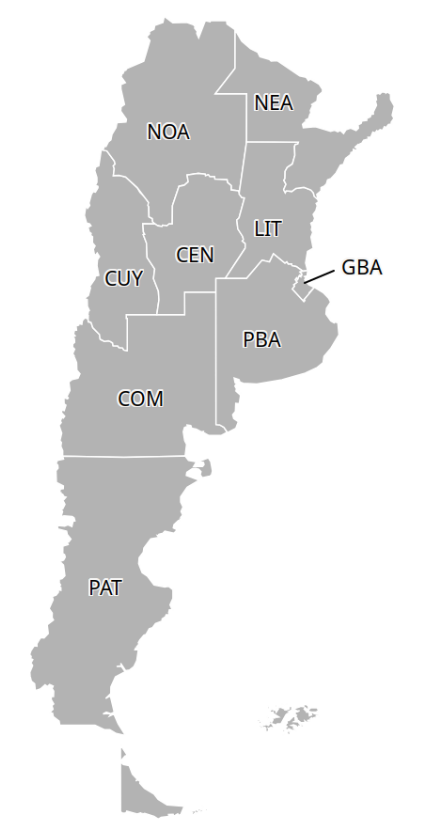
\includegraphics[width=6cm]{./Figures/regiones_electricas.png}
	\caption{Regiones eléctricas del SADI según definición utilizada por CAMMESA.}
	\label{fig:regiones_electricas}
\end{figure}

El SOTR provee medidores de demanda por regiones, pero no son aptos para el pronóstico de demanda debido a que no incluyen las pérdidas que se producen en las líneas eléctricas que vinculas las regiones. Por este motivo, fue necesario desarrollar un algoritmo que obtenga los valores de generación e intercambios de cada región y, realizando la sumatoria correspondiente, calcule la demanda. Por otra parte, se hizo una repartición de las pérdidas entre corredores, asignando la mitad a cada una de las regiones asociadas al vínculo.

Para expresarlo de forma matemático, sea \(G_r\) la generación de la región \(r\), \(\mathcal{N}_r\) el conjunto de
regiones vinculadas y \(F_{r\rightarrow j}\) y \(F_{j\rightarrow r}\) las
mediciones del intercambio en ambos extremos del corredor. La demanda regional
se calcula haciendo:

\begin{equation}
	D_r =
	G_r -
	\sum_{j \in \mathcal{N}_r}
	\frac{F_{r\rightarrow j}-F_{j\rightarrow r}}{2}
	\label{eq:demanda_regional}
\end{equation}

donde los intercambios son positivos cuando representan una exportación desde
la región \(r\). La semidiferencia entre las mediciones de ambos extremos
permite repartir las pérdidas del corredor en partes iguales entre las regiones
vinculadas.

La figura \ref{fig:regiones_electricas_sotr}, tomada del SOTR, muestra el estado de generación e intercambio entre algunas regiones para un instante determinado.

\begin{figure}[H]
	\centering
	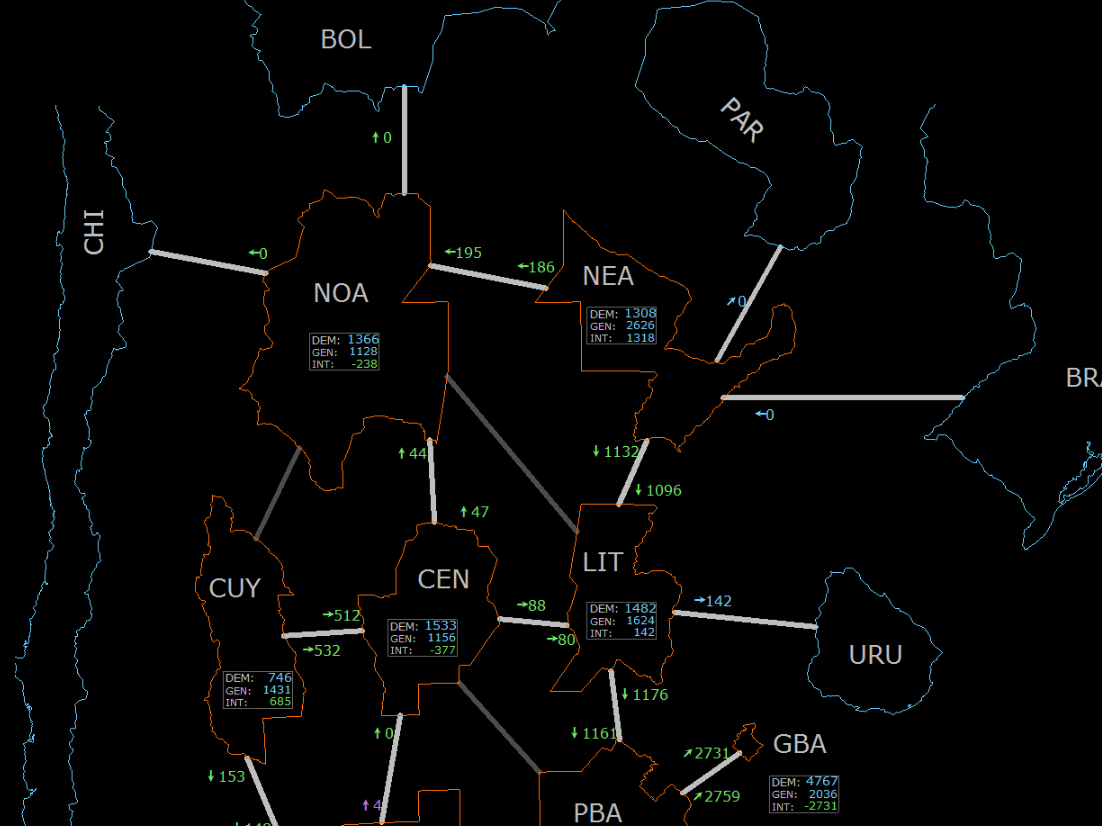
\includegraphics[width=\textwidth]{./Figures/regiones_electricas_sotr.png}
	\caption{Generación e intercambios entre regiones. Imagen del SOTR de CAMMESA para un instante determinado.}
	\label{fig:regiones_electricas_sotr}
\end{figure}

Si utilizamos la fórmula anterior para calcular la demanda corregida por pérdidas para LIT, podemos hacer (el intercambio con Uruguay es igual en ambos extremos, ya que es un vinculo interno de la central Salto Grande):

\begin{equation}
	\begin{aligned}
		D_{\mathrm{LIT}}
		={}& 1624
		-\left[
		\frac{-1096-1132}{2}
		+\frac{-80-88}{2}
		\right. \\
		&\left.
		+\frac{142-(-142)}{2}
		+\frac{1176-(-1161)}{2}
		\right] 
	\end{aligned}
	\label{eq:demanda_lit}
\end{equation}


Resolviendo,

\begin{equation}
	D_{\mathrm{LIT}}
	=
	1624-
	\left(-1114-84+142+1168{,}5\right)
	=
	1511{,}5~\mathrm{MW}
\end{equation}

Notar que el valor obtenido de 1511,5 MW difiere de los 1482 MW de demanda sin considerar las pérdidas. En caso de no aplicar esta corrección, la demanda nacional agregada presentaría un error considerable introducido en los datos de entrenamiento de los modelos.

La implementación de esta corrección requirió definir todos los intercambios entre regiones y consultar una cantidad de medidores del SOTR sustancialmente mayor que si se hubiesen podido utilizar los medidores de demanda existentes.

Por otra parte, se aplican ajustes específicos para representar de forma consistente la demanda utilizada en la programación. Entre ellos se encuentran la exclusión de consumos asociados con centrales de bombeo, que se ponen en servicio para almacenamiento de energía, y la demanda de grandes acerías que informan su consumo previsto.

El proceso genera también variables de control. La demanda MEM calculada como suma de las regiones se compara con un medidor nacional de referencia. Se almacenan la diferencia absoluta y porcentual entre ambos valores. Para PBA se conservan la demanda original, los valores directos de PBN y PBS y las diferencias asociadas con la partición. Asimismo, se calcula la suma de los intercambios internos, que debe permanecer próxima a cero porque las exportaciones de una región son importaciones de otra. Estos campos no constituyen objetivos de pronóstico, pero permiten verificar la coherencia del cálculo y detectar cambios en los medidores o en las reglas de negocio.

La salida se persiste en la tabla \code{DEMANDA.DEMANDA\_REGIONES\_10M}. Su clave está formada por fecha, hora e intervalo. Las columnas de demanda se almacenan en formato ancho, con una columna por región, junto con MEM y las variables de control. Esta tabla actúa como fuente para los procesos que generan resoluciones horarias y diarias.

La tarea de Dagster que ejecuta este proceso está programada cada 20 minutos, con el objetivo de mantener la tabla lo suficientemente actualizada para cualquier otro uso.

%----------------------------------------------------------------------------------------
\subsection{Transformación de demanda de diez minutos a resolución horaria}
\label{subsec:demanda_10m_1h}
%----------------------------------------------------------------------------------------

La transformación horaria se implementó en un notebook de Fabric. El proceso lee la tabla de diez minutos, controla la disponibilidad de nuevos registros y procesa únicamente el intervalo necesario. Para admitir correcciones tardías en la fuente se vuelve a considerar el día anterior al último registro persistido. Si no existen horas nuevas completas, el notebook finaliza sin efectuar escrituras.

Una hora se considera completa cuando contiene los seis intervalos esperados de diez minutos. Este criterio evita calcular promedios horarios a partir de observaciones parciales. Luego, la tabla en formato ancho se transforma a formato largo, con una fila por fecha, hora y región. La transformación facilita aplicar reglas homogéneas de limpieza y vincular cada observación con la dimensión de regiones.

La limpieza se realiza en dos etapas. Primero se identifican valores extremos por región mediante el rango intercuartílico. Los límites se establecen a partir del primer y tercer cuartil y un factor de tres veces el rango intercuartílico. Los valores que quedan fuera de esos límites se reemplazan temporalmente por valores nulos y se estiman mediante interpolación lineal en el eje temporal. En la figura \ref{fig:correccion_outliers} puede verse un caso de corrección de valores extremos.

El método de eliminación de outliers es eficiente para fallas de medición, donde se alcanzan valores extremos por instantes cortos de tiempos. Las correcciones más desafiantes son aquellas que corresponden a fallas eléctricas reales del sistema eléctrico (por ejemplo, la desconexión intempestiva de una línea de transmisión que hace caer la demanda abruptamente). En estos casos, es deseable poder inferir el valor de demanda si no hubiese existido la falla, ya que, a los fines del entrenamiento de un modelo predictivo, esto representa un error que debe ser desestimado.

Por este motivo, en la segunda etapa se detectan escalones abruptos dentro de un mismo día. Un cambio se considera candidato a corrección cuando supera simultáneamente un umbral relativo del 7\% y un umbral absoluto de 100~MW. Estos valores fueron determinados en base a la recomendación de los especialistas de CAMMESA en combinación con el análisis de amplios rangos temporales. La detección y corrección se ejecuta de manera iterativa, con un máximo de diez iteraciones. Los puntos identificados se interpolan y, cuando la interpolación no resulta posible en los extremos, se completan mediante propagación hacia adelante o hacia atrás. En la figura \ref{fig:correccion_saltos_bruscos} puede verse un caso de corrección de saltos bruscos.

\begin{figure}[H]
	\centering
	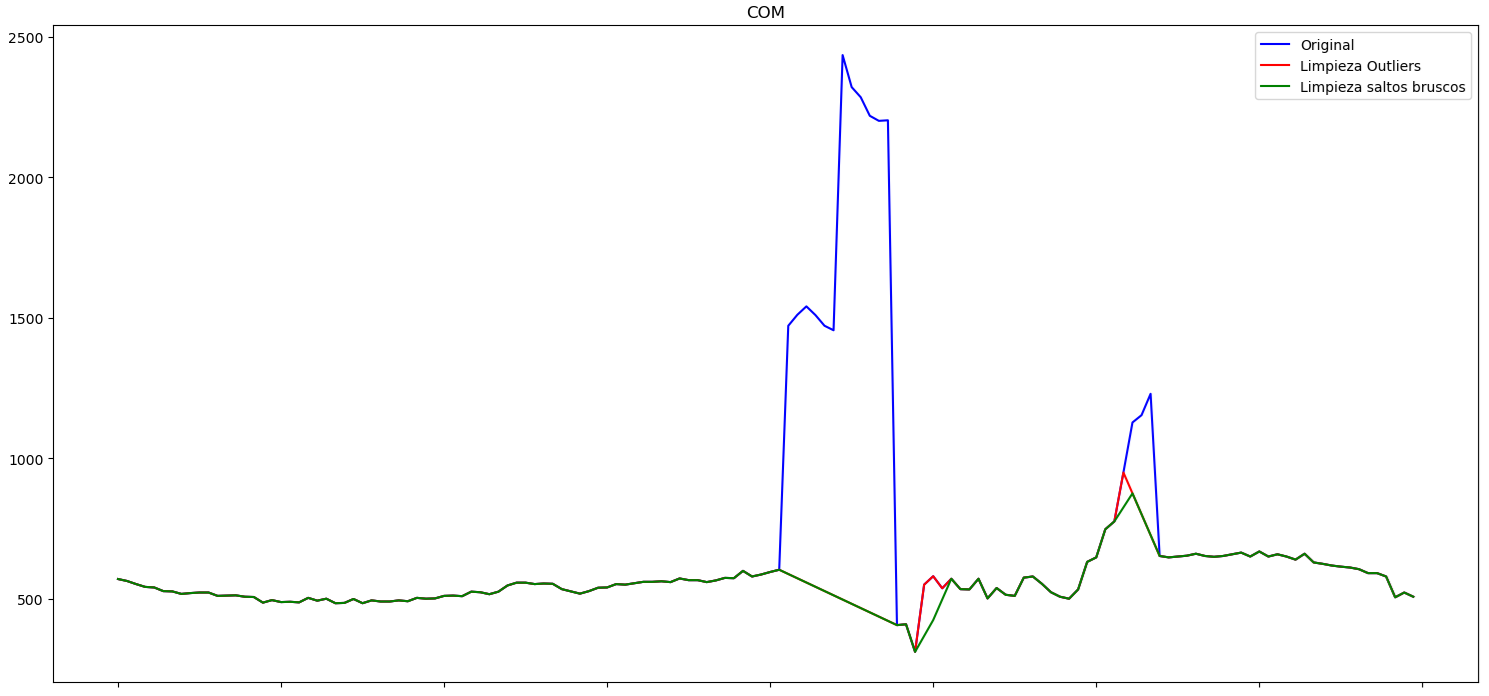
\includegraphics[width=\textwidth]{./Figures/correccion_outliers.png}
	\caption{Corrección de valores extremos.}
	\label{fig:correccion_outliers}
\end{figure}

\begin{figure}[H]
	\centering
	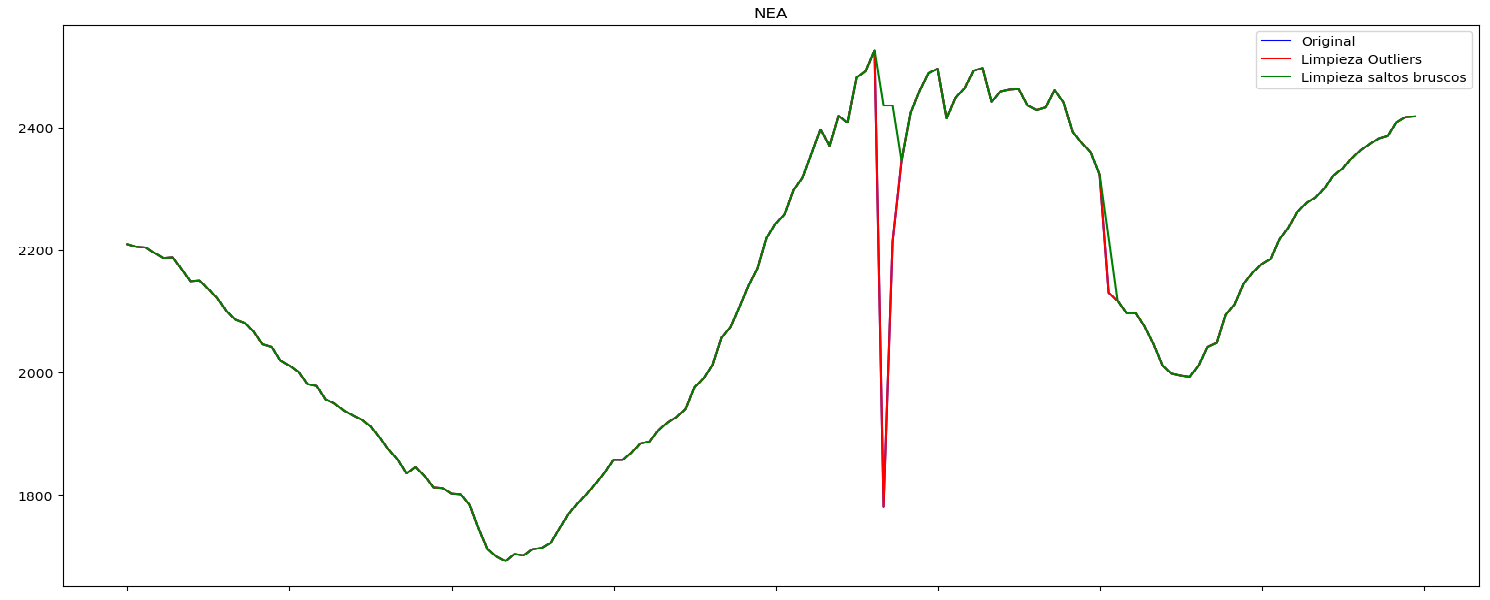
\includegraphics[width=\textwidth]{./Figures/correccion_saltos_bruscos.png}
	\caption{Corrección de saltos bruscos.}
	\label{fig:correccion_saltos_bruscos}
\end{figure}

Después de la limpieza se calcula el promedio de los seis registros de cada hora. Se conservan tanto el valor resultante como el promedio obtenido a partir de los datos anteriores a la corrección. La columna \code{FLAG\_CORREGIDO} indica si ambos valores difieren. De este modo, los modelos pueden utilizar la serie depurada sin perder la posibilidad de auditar qué observaciones fueron modificadas.

Cada registro se vincula con la dimensión regional mediante la clave \code{RGE\_ID} y el período de vigencia correspondiente. La tabla final contiene \code{FECHA}, \code{HORA}, \code{RGE\_ID}, \code{VALOR}, \code{FLAG\_CORREGIDO} y \code{VALOR\_ORIGINAL}. Antes de persistir, se verifica la existencia de la clave compuesta en el destino para evitar duplicados. Los registros nuevos se incorporan en \code{DEMANDA.DEMANDA\_REGIONES\_1H}.

A partir de la demanda horaria se obtienen variables diarias utilizadas como objetivos. La energía diaria se almacena por región en la tabla del esquema DEMANDA llamada \code{DEMANDA\_REGIONES\_DIARIA}. Las vistas del Warehouse suman los valores regionales para obtener la demanda del MEM y calculan las potencias máxima y mínima sobre los intervalos horarios definidos para cada variable. Esta derivación mantiene una fuente regional común para los objetivos nacionales y permite comprobar que el agregado del MEM sea consistente con sus componentes.

%----------------------------------------------------------------------------------------
\subsection{Ingesta y procesamiento de datos meteorológicos reales}
\label{subsec:pipeline_meteorologico}
%----------------------------------------------------------------------------------------

El flujo meteorológico integra observaciones del Servicio Meteorológico Nacional y valores obtenidos de Open-Meteo. La primera etapa se ejecuta en el notebook \code{NB\_METEO\_L1}. Para el SMN se procesan los archivos de observaciones diarias y de datos horarios. Para Open-Meteo se realizan consultas por coordenadas asociadas con estaciones de referencia. El rango de fechas se recibe como parámetro y, cuando no se informa, el notebook utiliza el día anterior a la ejecución.

Los archivos descargados del SMN se conservan en un Lakehouse. Esta copia permite mantener el insumo original y volver a procesarlo si resulta necesario. Los datos interpretados se escriben en la base KQL \code{EH\_PSYD}, utilizada como capa~1. Allí se almacenan, entre otras variables, temperatura, humedad relativa, presión, dirección y velocidad del viento para la resolución horaria, y temperaturas máxima y mínima para la resolución diaria. Las tablas de Open-Meteo incorporan además temperatura aparente, nubosidad, precipitación y radiación solar, según la resolución de cada conjunto.

La persistencia en KQL se realiza por lotes. Antes de insertar un período se eliminan los registros existentes para el mismo rango temporal. Esta estrategia permite repetir una ejecución sin conservar versiones duplicadas del mismo dato. Cuando el volumen serializado supera el tamaño previsto para una operación, la carga se divide en bloques. El resultado de esta etapa es una representación cercana a las fuentes, separada por proveedor y resolución.

La transferencia desde la capa~1 hacia la capa~2 se orquesta mediante el Pipeline \code{PPLN\_METEO}, que se presenta en la figura \ref{fig:pipeline_meteo}. El pipeline ejecuta el notebook y consulta en el Warehouse las estaciones cuya vigencia se superpone con el período procesado. Esta validación evita incorporar estaciones que no correspondan al intervalo analizado y permite asociar cada nombre de estación con su identificador \code{EMET\_ID}.

\begin{figure}[H]
	\centering
	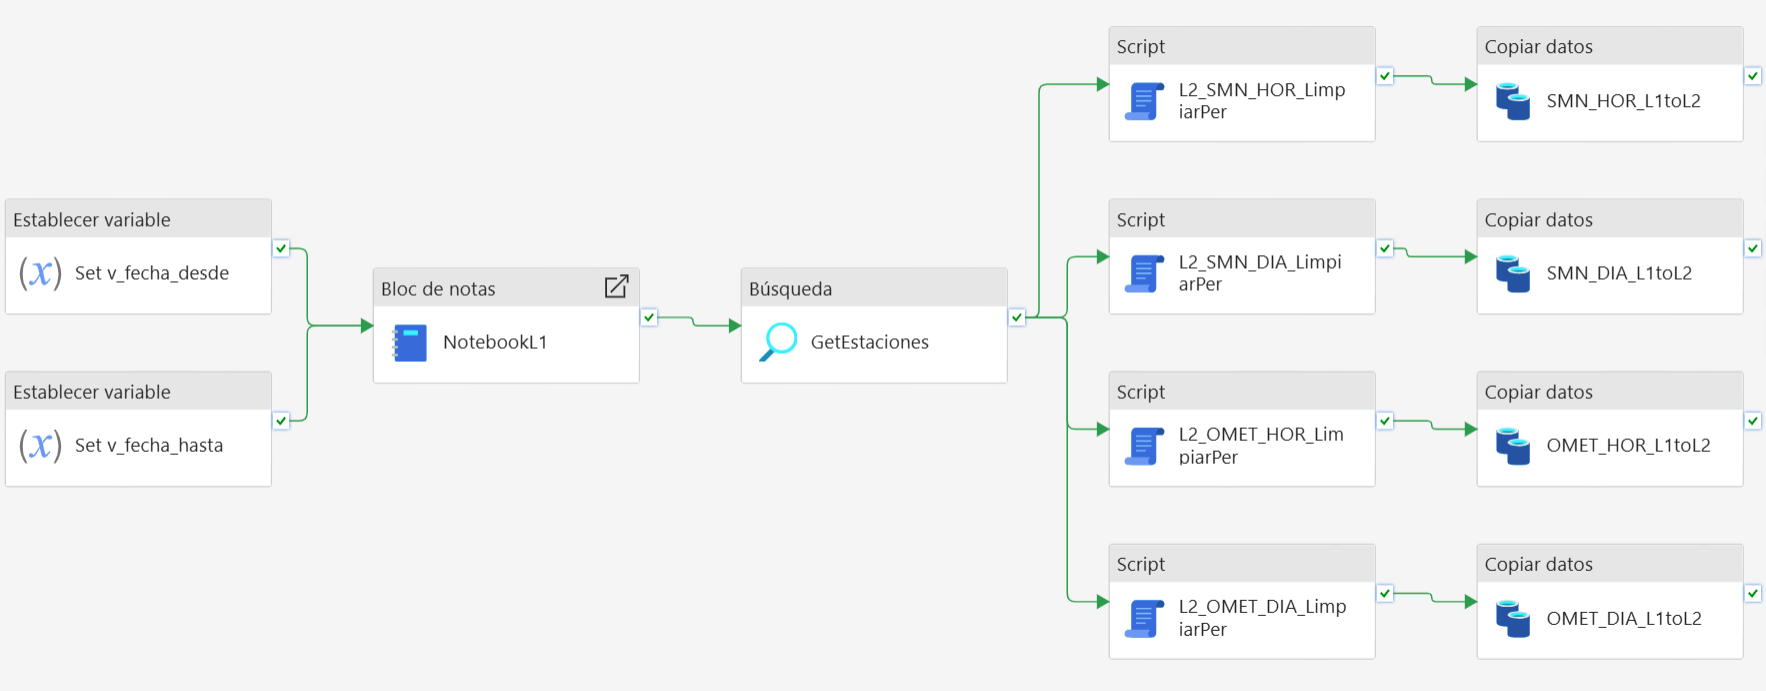
\includegraphics[width=\textwidth]{./Figures/pipeline_meteo.png}
	\caption{Pipeline de Fabric para la orquestación de datos meteorológicos.}
	\label{fig:pipeline_meteo}
\end{figure}

Para los datos horarios del SMN, la actividad de copia filtra el rango de fechas, conserva las estaciones vigentes y construye la marca temporal \code{FECHA\_HORA}. También ajusta la numeración horaria para compatibilizarla con la convención utilizada en CAMMESA. A partir de la temperatura, la humedad relativa y la velocidad del viento se calcula una temperatura aparente. Finalmente, las variables se redondean y tipifican antes de escribirlas en el esquema \code{METEO} del Warehouse.

La escritura de los datos meteorológicos utiliza claves temporales y de estación. Para los valores horarios, la combinación de \code{FECHA\_HORA} y \code{EMET\_ID} identifica cada observación. Las tablas diarias emplean la fecha y el identificador de estación. Esta estructura permite comparar proveedores para una misma ubicación, seleccionar estaciones representativas de cada región eléctrica y construir agregados diarios sin perder el origen del dato.

%%----------------------------------------------------------------------------------------
%\subsection{Integración y disponibilidad para el modelado}
%\label{subsec:integracion_modelado}
%%----------------------------------------------------------------------------------------
%
%Una vez procesados ambos flujos, la demanda y la meteorología quedan disponibles en el Data Warehouse con claves temporales y geográficas explícitas. La dimensión de regiones vincula las series eléctricas con las estaciones meteorológicas mediante identificadores y períodos de vigencia. Esta relación es necesaria porque la disponibilidad de una estación y su representatividad regional pueden variar con el tiempo.
%
%La preparación de los conjuntos de modelado parte de las tablas horarias y diarias de capa~2. Para los modelos diarios se utilizan como variables objetivo la energía y las potencias mínima y máxima. Las variables explicativas se construyen a partir de la historia de la demanda, los registros meteorológicos y la información calendaria. La agregación se realiza después de los controles de calidad, de modo que un valor incompleto o anómalo no se propague sin identificación hacia los conjuntos de entrenamiento.
%
%La separación entre datos originales, datos corregidos y variables derivadas aporta trazabilidad al proceso. Los campos de control de la demanda regional permiten comprobar la conservación del balance nacional, mientras que \code{FLAG\_CORREGIDO} identifica las horas modificadas durante la limpieza. En meteorología, la conservación de los archivos originales del SMN y la capa inicial en KQL permiten revisar la transformación aplicada antes de la carga relacional.
%
%El pipeline implementado resuelve así la adquisición y preparación de las principales fuentes requeridas por el sistema de pronóstico. La automatización disminuye la dependencia de cargas manuales y establece una base común para comparar modelos bajo los mismos datos y reglas de procesamiento. Las etapas posteriores del capítulo describen la arquitectura de los modelos, el procedimiento de entrenamiento y su integración con los mecanismos de ejecución y seguimiento.